\newpage
\changeindent{0cm}
\section{数値実験}
\label{sec:exp}
\changeindent{2cm}


\changeindent{0cm}
\subsection{実験 1}
\label{sec:exp.01}
\changeindent{2cm}


\changeindent{0cm}
\subsubsection{実験概要}
\label{sec:exp.01_01}
\changeindent{2cm}

提案手法 : DARTS の実験を 実験 1 とする.
表 \ref{tab:setting_exp}, \ref{tab:exp2/eval} に実験 1 の探索段階と評価段階の実験設定を示す.
探索段階は先行研究の DARTS の設定を参考に, 評価段階は Optuna で最適化した値を使用した.
$\bm{\alpha}$ の Optimizer は Adam\cite{Kingma2015AdamAM} で,
評価段階では, 訓練中に学習率を変化させる Scheduler\cite{Loshchilov2017SGDRSG} を用いた.

データセットは, 32 pixel $\times$ 32 pixel $\times$ 3 channel の訓練画像を 50000 枚 持つ CIFAR-10\cite{cifar10} を利用して,
10 クラス分類問題を解いた.

探索 epoch 数は, 150 epochとし, 50 epochごとにその時点の $\bm{\alpha}$ の性能を評価した.
構成段階では手法 A, B に加えて比較のため,
ショートカット数が同じとなる条件でランダムに選択する手法でも実験した.
各手法において 10 回試行して統計的な性能を比較した.

\clearpage
\begin{table}[tb]
  \begin{center}
    \caption{実験 1 : 探索段階の設定}
  	\vspace{3mm}
    \begin{tabular}{|c|c|} \hline
      Step & Architecture Search \\ \hline\hline
      Loss & Cross Entropy Loss \\ \hline
      batch size & 64 \\ \hline
      Optimizer ($\bm{w}$) & SGD (lr = 0.001, momentum = 0.9) \\ \hline
      Optimizer ($\bm{\alpha}$) & Adam (lr = 0.003, $\bm{\beta}$ = (0.5, 0.999)) \\ \hline
      epoch & 150\\ \hline
      train data & 25000\\ \hline
      valid data & 25000\\ \hline
      test data &  10000\\ \hline
    \end{tabular}
    \label{tab:setting_exp}
  \end{center}
\end{table}

\begin{table}[tb]
  \begin{center}
    \caption{実験 1 : 評価段階の設定}
  	\vspace{3mm}
    \begin{tabular}{|c|c|} \hline
      Step & Evaluation \\ \hline\hline
      Loss & Cross Entropy Loss \\ \hline
      batch size & 64 \\ \hline
      Optimizer ($\bm{w}$) & SGD (lr = 0.0090131, momentum = 0.9) \\ \hline
      Scheduler ($\bm{w}$) & Step ($\gamma$ = 0.23440, stepsize = 100) \\ \hline
      epoch & 150\\ \hline
      train data & 50000\\ \hline
      test data &  10000\\ \hline
    \end{tabular}
    \label{tab:exp2/eval}
  \end{center}
\end{table}


\clearpage
\changeindent{0cm}
\subsubsection{結果}
\label{sec:exp.01_02}
\changeindent{2cm}



表 \ref{tab:accg} に各構成手法におけるテストデータの精度を示す.
図 \ref{fig:short}, \ref{fig:param} には
表 \ref{tab:accg} の精度に対するショートカット数とパラメータ数の関係を図示する.
最も性能が高かったのは 100 epoch 時点の手法 A で 94.02 \% (baseline + 0.99\%) となり,
100 epoch 時点の手法 B は 93.93 \% (baseline + 0.90\%) となった.
しかしランダム手法と比較すると, 手法 A は + 0.35 \%, 手法 B は + 0.46 \% となり,
図 \ref{fig:param} を参照しても少ないパラメータ数でより有効に探索できているのは手法 B と言える.

また 100 epoch 時点と 150 epoch 時点を比較すると, 150 epoch の方が性能が悪化していることが分かる.
問題に対して過度に適合していることが原因であると考えられる.

探索時間は 150 epoch でおよそ 5 GPU hours を要したが,
先行研究の DARTS では 3 GPU days であった.
先行研究と比べ演算子を探索していないことや.
最適な重み $\bm{w}$ の近似を 1 次下げていることで高速になったと思われる.

% ここで 0.5 Page


\begin{table}[tb]
  \begin{center}
    \caption{実験 1 : 各アーキテクチャの精度}
		\vspace{3mm}
    \begin{tabular}{|c|c|c|c|c|c|}\hline
    \multicolumn{2}{|c|}{\textbf{architecture}} & \textbf{\begin{tabular}[c]{@{}c@{}}test accuracy\\ (\%)\end{tabular}} & \textbf{\begin{tabular}[c]{@{}c@{}}param\\ (M)\end{tabular}} & \textbf{\begin{tabular}[c]{@{}c@{}}shortcut \# \end{tabular}} & \textbf{\begin{tabular}[c]{@{}c@{}}random architect\\ accuracy (\%)\end{tabular}} \\ \hline
    \multirow{3}{*}{\begin{tabular}[c]{@{}c@{}}method A\end{tabular}} & 50 epoch & 93.70 $\pm$ 0.22 & 21.06 $\pm$ 0.07 & 12.7 $\pm$ 1.4 & 93.60 $\pm$ 0.15 \\ \cline{2-6}
     & 100 epoch & 94.02 $\pm$ 0.12 & 21.50 $\pm$ 0.11 & 18.2 $\pm$ 0.9 & 93.67 $\pm$ 0.14 \\ \cline{2-6}
     & 150 epoch & 93.90 $\pm$ 0.17 & 21.57 $\pm$ 0.25 & 18.9 $\pm$ 0.6 & 93.64 $\pm$ 0.09 \\ \hline
    \multirow{3}{*}{\begin{tabular}[c]{@{}c@{}}method B\end{tabular}} & 50 epoch & 93.57 $\pm$ 0.19 & 20.45 $\pm$ 0.09 & 5.8 $\pm$ 1.2 & 93.36 $\pm$ 0.19 \\ \cline{2-6}
     & 100 epoch & 93.93 $\pm$ 0.08 & 20.73 $\pm$ 0.10 & 9.8 $\pm$ 1.0 & 93.47 $\pm$ 0.17 \\ \cline{2-6}
     & 150 epoch & 93.92 $\pm$ 0.12 & 20.76 $\pm$ 0.15 & 10.6 $\pm$ 1.0 & 93.48 $\pm$ 0.15 \\ \hline
    \multicolumn{2}{|c|}{baseline (VGG19)} & 93.03 $\pm$ 0.10 & 20.04 & 0 & - \\ \hline
    \end{tabular}
    \label{tab:accg}
  \end{center}
\end{table}


\begin{figure}[t]
  \begin{tabular}{c}
    \begin{minipage}[t]{0.95\hsize}
    	\begin{center}
        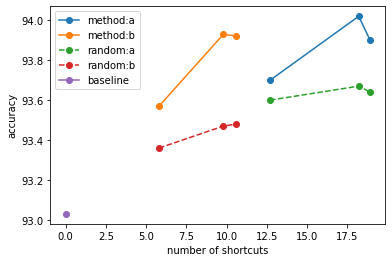
\includegraphics[clip, width=95mm]{./fig/short.png}
      \end{center}
      \caption{実験 1 : ショートカット数に対する精度}
      \label{fig:short}
    \end{minipage}
    \vspace{3cm}
    \\
    \begin{minipage}[c]{0.95\hsize}
      \begin{center}
        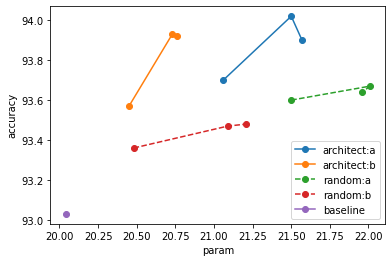
\includegraphics[clip,width=95mm]{./fig/param.png}
      \end{center}
      \caption{実験 1 : パラメータ数に対する精度}
      \label{fig:param}
    \end{minipage}
  \end{tabular}
\end{figure}


% \clearpage
% \begin{figure}[t]
%   \begin{center}
%     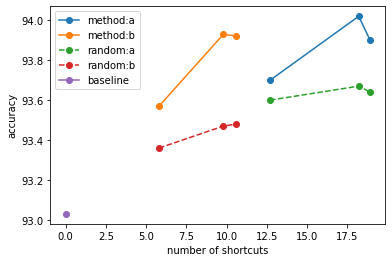
\includegraphics[clip,width=10cm]{./fig/short.png}
%   \end{center}
%   \caption{実験1 : ショートカット数に対する精度}
%   \label{fig:short}
% \end{figure}
% \begin{figure}[t]
%   \begin{center}
%     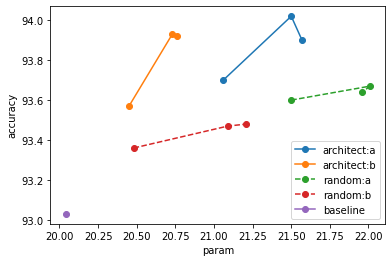
\includegraphics[clip,width=10cm]{./fig/param.png}
%   \end{center}
%   \caption{実験1 : パラメータ数に対する精度}
%   \label{fig:param}
% \end{figure}


図 \ref{fig:exp1_a}, \ref{fig:exp1_b} には, 手法 A, B のアーキテクチャの 50 epoch ごとの
結果として, 10 回試行のうちの 1 つを示した.
ランダム探索では見られなかったような, 比較的離れた位置からの接続が多いという特徴があった.
さらに, 学習を経るごとに離れていくため, 接続の距離がネットワークの性能に関係していると考えられる.
これは離れた位置からの接続が, あまり変換されていない特徴の情報を引き継げることによって
性能が向上したと解釈できる.



\begin{figure}[tb]
 \begin{minipage}{0.3\hsize}
 	\begin{center}
 		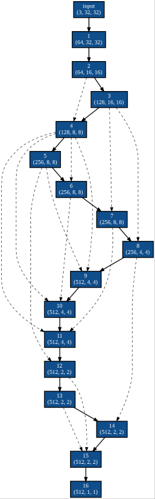
\includegraphics[clip,scale=0.8]{./fig/04.exp/a50.png}\\
 		50 epoch
 	\end{center}
 \end{minipage}
 \begin{minipage}{0.3\hsize}
 	\begin{center}
    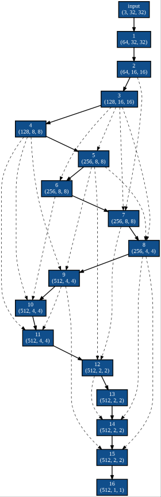
\includegraphics[clip,scale=0.8]{./fig/04.exp/a100.png}\\
    100 epoch
 	\end{center}
 \end{minipage}
 \begin{minipage}{0.3\hsize}
 	\begin{center}
    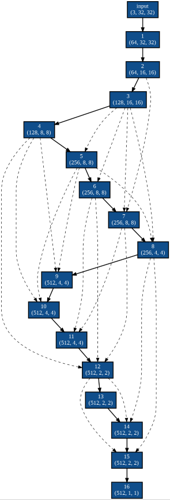
\includegraphics[clip,scale=0.8]{./fig/04.exp/a150.png}\\
    150 epoch
 	\end{center}
 \end{minipage}
 \caption{実験 1 : 手法 A のアーキテクチャ 例}
 \label{fig:exp1_a}
\end{figure}


\begin{figure}[tb]
 \begin{minipage}{0.3\hsize}
 	\begin{center}
 		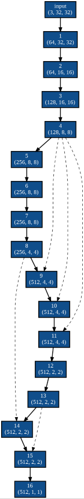
\includegraphics[clip,scale=0.8]{./fig/04.exp/b50.png}\\
 		50 epoch
 	\end{center}
 \end{minipage}
 \begin{minipage}{0.3\hsize}
 	\begin{center}
    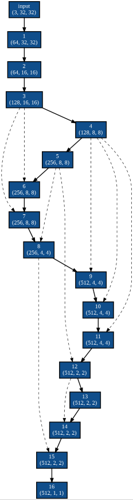
\includegraphics[clip,scale=0.8]{./fig/04.exp/b100.png}\\
    100 epoch
 	\end{center}
 \end{minipage}
 \begin{minipage}{0.3\hsize}
 	\begin{center}
    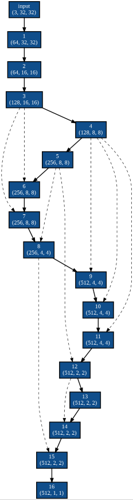
\includegraphics[clip,scale=0.8]{./fig/04.exp/b150.png}\\
    150 epoch
 	\end{center}
 \end{minipage}
 \caption{実験 1 : 手法 B のアーキテクチャ 例}
 \label{fig:exp1_b}
\end{figure}










\clearpage\newpage
\changeindent{0cm}
\subsection{実験 2}
\label{sec:exp.02}
\changeindent{2cm}



\changeindent{0cm}
\subsubsection{実験概要}
\label{sec:exp.02_01}
\changeindent{2cm}

提案手法 : DARTS + TDGA の実験を 実験 2 とする.

表 \ref{tab:setting_pretrain} には事前学習の設定を示した.
実験 1 の設定を継承しつつ,
モデルの重み $\bm{w}$ は Image Net\cite{deng2009imagenet} で訓練された
事前学習の重みを畳み込み層の部分に適用した.

表 \ref{tab:setting_darts}, \ref{tab:setting_ga}にモデルと GA の実験設定を示した.
初期収束を防ぐため, 交叉にはエッジに相当する遺伝子座ごとに 0.8 の確率で操作する一様交叉を使用した.
突然変異には遺伝子座ごとに 0.1 の確率で $\mu=0$, $\gamma=0.2$ となるガウス分布からの摂動を与えた.
交叉と突然変異の操作確率は, 個体ごとの確率で, それぞれは独立であり, 交叉の後に突然変異をした.

% ここで 0.5 Page

\begin{table}[tb]
  \begin{center}
    \caption{実験 2 : 事前学習の設定}
  	\vspace{3mm}
    \begin{tabular}{|c|c|} \hline
      Optimizer ($\bm{w}$) & SGD (lr = 0.001, momentum = 0.9) \\ \hline
      Optimizer ($\bm{\alpha}$) & Adam (lr = 0.0005, $\bm{\beta}$ = (0.5, 0.999)) \\ \hline
      Loss & Cross Entropy Loss \\ \hline
      batch size & 64 \\ \hline
      train data & 25000\\ \hline
      valid data & 25000\\ \hline
      test data &  10000\\ \hline
      epoch & 150\\ \hline
    \end{tabular}
    \label{tab:setting_pretrain}
  \end{center}
\end{table}

\begin{table}[t]
  \begin{center}
    \caption{実験 2 : DARTS + TDGAの設定 (DARTS)}
  	\vspace{3mm}
    \begin{tabular}{|c|c|} \hline
      Optimizer ($\bm{w}$) & SGD (lr = 0.001, momentum = 0.9) \\ \hline
      Optimizer ($\bm{\alpha}$) & Adam (lr = 0.001, $\bm{\beta}$ = (0.5, 0.999)) \\ \hline
      Loss & Cross Entropy Loss \\ \hline
      batch size & 64 \\ \hline
      train data & 25000\\ \hline
      valid data & 25000\\ \hline
      test data &  2000\\ \hline
    \end{tabular}
    \label{tab:setting_darts}
  \end{center}
\end{table}

\begin{table}[t]
  \begin{center}
    \caption{実験 2 : DARTS + TDGAの設定 (TDGA)}
  	\vspace{3mm}
    \begin{tabular}{|c|c|} \hline
      Population & 10 \\ \hline
      Generation & 150 \\ \hline \hline
      Selection & Elite \\ \hline
      Elite \# & 1 \\ \hline
      Selection & TD Select \\ \hline
      Temperature & 1 $\rightarrow$ 0.001 \\ \hline \hline
      Crossover & Uniform Crossover (0.5 / locus) \\ \hline
      Crossover Rate & 0.8 \\ \hline \hline
      Mutation & Gaussian Mutation ($\mu$ = 0, $\sigma$ = 0.2, 0.2 / locus)\\ \hline
      Mutation Rate & 0.2 \\ \hline
    \end{tabular}
    \label{tab:setting_ga}
  \end{center}
\end{table}

\begin{table}[t]
  \begin{center}
    \caption{実験 2 : ネットワーク評価の設定}
  	\vspace{3mm}
    \begin{tabular}{|c|c|} \hline
      Optimizer ($\bm{w}$) & SGD (lr = 0.009, momentum = 0.9) \\ \hline
      Scheduler ($\bm{w}$) & Step ($\gamma$ = 0.2344, step epoch = 100) \\ \hline
      Loss & Cross Entropy Loss \\ \hline
      batch size & 64 \\ \hline
      train data & 50000\\ \hline
      test data &  10000\\ \hline
      epoch & 150\\ \hline
    \end{tabular}
    \label{tab:setting_eval}
  \end{center}
\end{table}


\clearpage
\changeindent{0cm}
\subsubsection{結果}
\label{sec:exp.02_02}
\changeindent{2cm}



表 \ref{tab:acc_ga} に, 3 つの提案手法の最終的なアーキテクチャ性能を示す.
50 世代ごとの結果全てに対して, DARTS のみとなる事前学習のアーキテクチャ 93.65 \% をいずれも超えている.
図 \ref{fig:exp2/eval} は 横軸に世代数, 縦軸に accuracy をとった,
表 \ref{tab:acc_ga} のグラフを示す.
$\bm{w}$ を更新する提案手法 1 が 150 世代目で性能が下がっている.
また DARTS の更新をしない提案手法 3 が最もよい結果となった.


\begin{table}[t]
  \begin{center}
    \caption{実験 2 : 各提案手法のアーキテクチャ性能}
		\vspace{-1mm}
    ベースラインは事前学習時のネットワーク.
		\vspace{1mm}
		\vspace{3mm}
    \begin{tabular}{|c|c|c|c|} \hline
    \textbf{}       & \textbf{50 世代} & \textbf{100 世代} & \textbf{150 世代} \\ \hline\hline
    DARTS + TDGA ($\bm{w}$, $\bm{\alpha}$)& 94.03 \%       & 94.10 \%        & 93.85 \%        \\ \hline
    DARTS + TDGA ($\bm{\alpha}$)& 93.88 \%       & 94.08 \%        & 94.13 \%        \\ \hline
    DARTS + TDGA   & 93.90 \%       & 94.17 \%        & 94.17 \%        \\ \hline
    Baseline (DARTS) & \multicolumn{3}{c|}{93.65 \%}                      \\ \hline
    \end{tabular}
    \label{tab:acc_ga}
  \end{center}
\end{table}

\begin{figure}[t]
  \begin{center}
    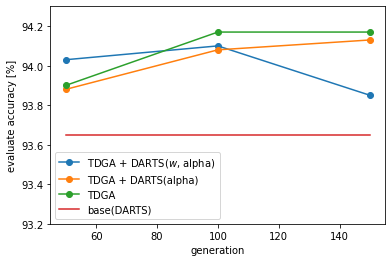
\includegraphics[clip,width=10cm]{./fig/04.exp/eval.png}
  \end{center}
  \caption{実験 2 : 各提案手法のアーキテクチャ性能}
  \label{fig:exp2/eval}
\end{figure}


次に 図 \ref{fig:exp2/acc} ~ \ref{fig:exp2/edge} で探索段階のデータを考察する.

図 \ref{fig:exp2/acc}, 図 \ref{fig:exp2/loss}に
提案手法の適応度計算時のテストデータの正解率と損失を示す.
ただし個体群の中で最良の適応度を得た個体をその世代の代表としている.
提案手法 1 は重み $\bm{w}$ も更新しているため, 最も訓練時の正解率が高く, 90 \% 付近まで学習している.
それと比べて, 提案手法 2, 3 は 10 \% 程度低くなっているが,
提案手法 3 は 提案手法 2 と比較して, 150 世代でも正答率の増加傾向が見られる.
図 \ref{fig:exp2/eval} の最終的な評価から考えて, 学習時の正答率の高さが
ネットワークの性能と直結しているわけではないことが分かった.
また 提案手法 2, 3 は $\bm{w}$ を固定しており, 同じ個体に対しては同じ適応度が計算されるため,
純粋にアーキテクチャが学習される過程を示している.
この同じ適応度が計算されるという信頼性が, 提案手法 2, 3 の結果が 提案手法 1 よりも優れていた
原因であると考えられる.
したがって適応度計算には, 学習過程の正答率よりも同じ結果となることがより重要であると言える.

図 \ref{fig:exp2/edge} には, 各探索段階での採用されるショートカット数を示した.
ただしショートカット数は最良個体のものとした.
提案手法 2, 3 は 世代数が 50 から 100 のときに主に改善されているが,
図 \ref{fig:exp2/edge} を参照するとショートカット数は減少している最中である.
ネットワークの計算の邪魔になる, 不必要な辺を削除できたことで性能が改善されたことが分かった.


\begin{figure}[t]
  \begin{center}
    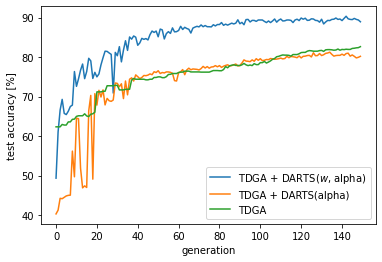
\includegraphics[clip,width=10cm]{./fig/04.exp/acc.png}
  \end{center}
  \caption{実験 2 : 各提案手法の探索時の正解率}
  \label{fig:exp2/acc}
\end{figure}
\begin{figure}[t]
  \begin{center}
    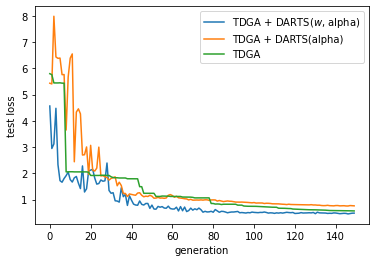
\includegraphics[clip,width=10cm]{./fig/04.exp/loss.png}
  \end{center}
  \caption{実験 2 : 各提案手法の探索時の損失}
  \label{fig:exp2/loss}
\end{figure}
\begin{figure}[t]
  \begin{center}
    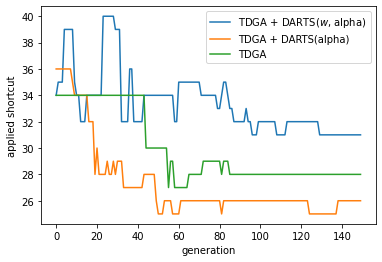
\includegraphics[clip,width=10cm]{./fig/04.exp/edge.png}
  \end{center}
  \caption{実験 2 : 各提案手法の探索過程のショートカット数}
  \label{fig:exp2/edge}
\end{figure}

図 \ref{fig:exp2/archi}, \ref{fig:exp2/archi2} には,
事前学習と各提案手法の最終世代時の最良個体のアーキテクチャを示した.
実験 1 でもみられたような離れた位置からのショートカットが多いという特徴が, 提案手法 2, 3 でもみられ,
逆に提案手法 1 では無秩序を感じさせるような様々な位置で接続する構造となった.


\begin{figure}[tb]
 \begin{minipage}{0.49\hsize}
 	\begin{center}
    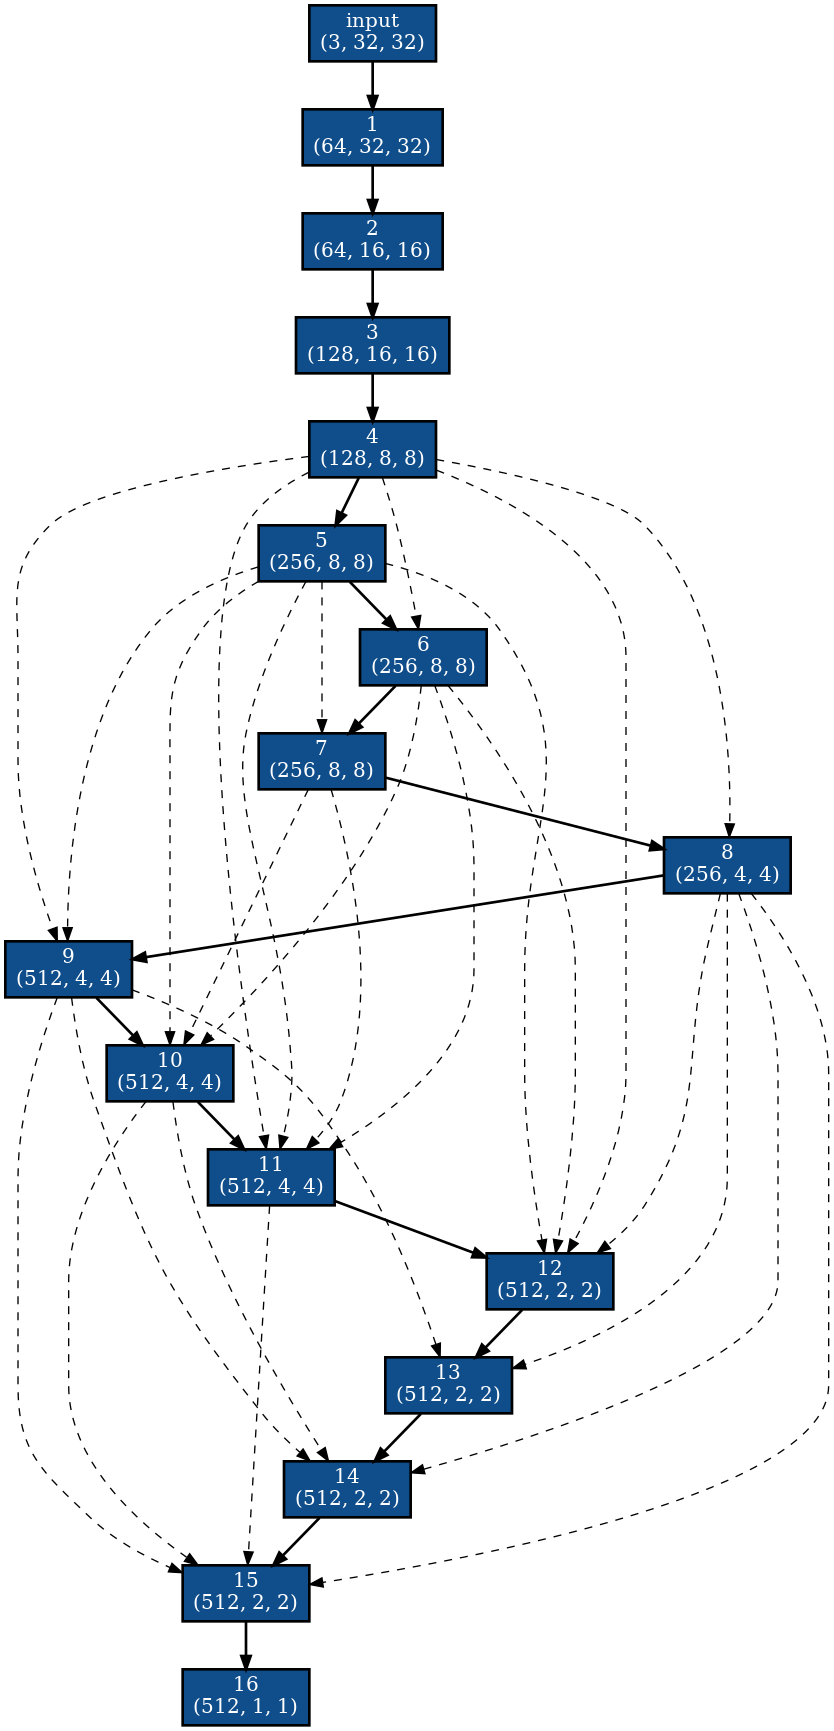
\includegraphics[clip,scale=0.2]{./fig/04.exp/base.png}\\
    Baseline (DARTS)
 	\end{center}
 \end{minipage}
 \begin{minipage}{0.49\hsize}
 	\begin{center}
    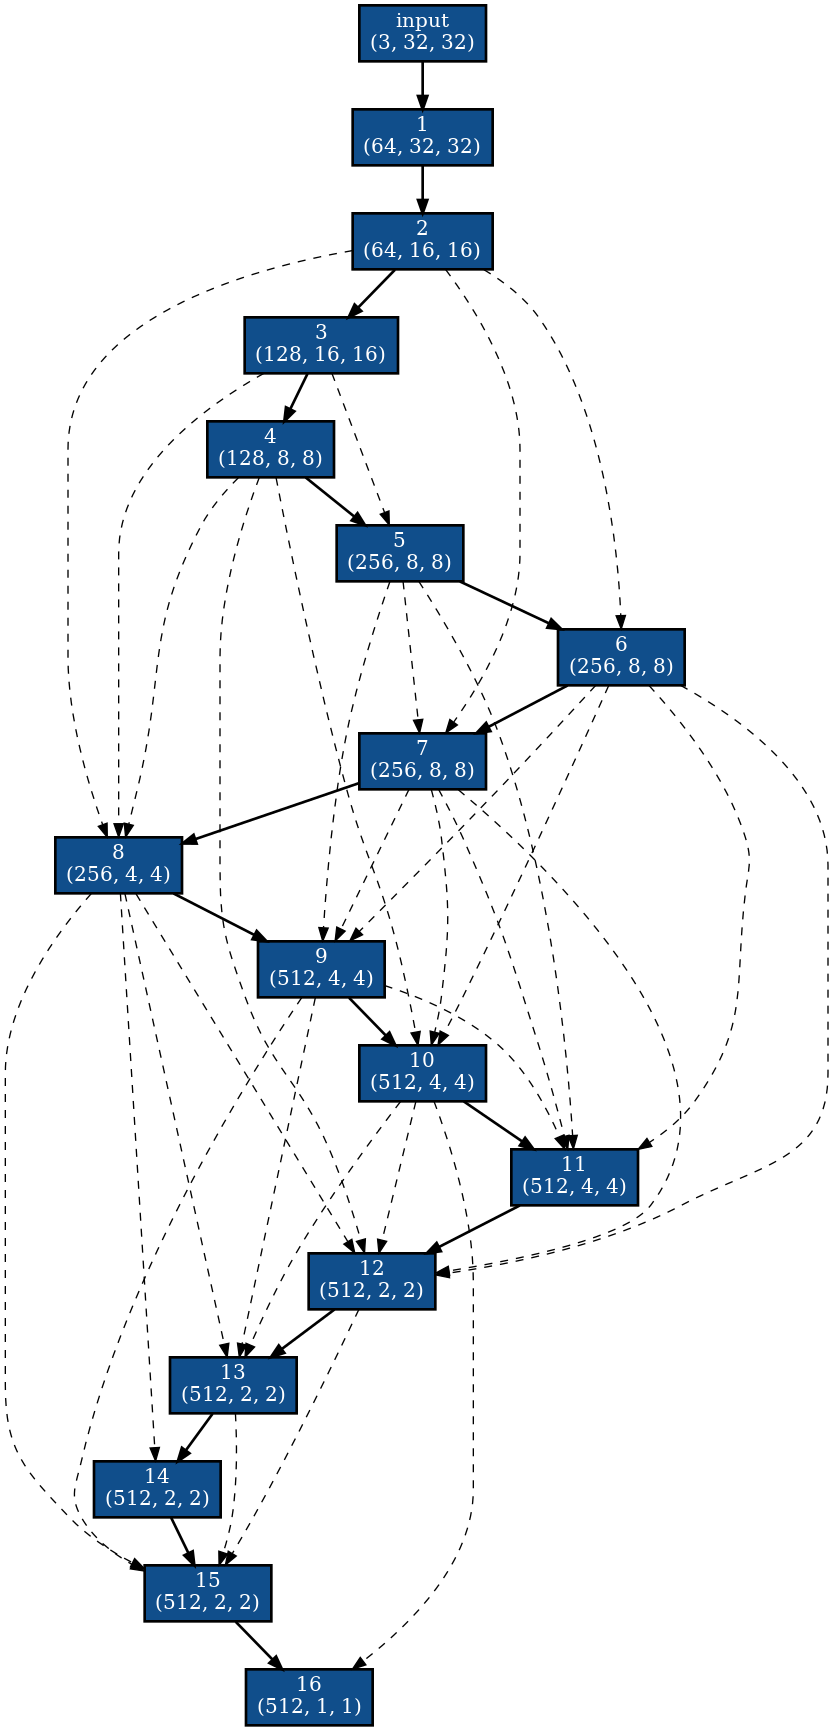
\includegraphics[clip,scale=0.2]{./fig/04.exp/nofix_last.png}\\
    DARTS + TDGA ($\bm{w}$, $\bm{\alpha}$)
 	\end{center}
 \end{minipage}
 \caption{実験 2 : 手法のアーキテクチャ 1 / 2}
 \label{fig:exp2/archi}
\end{figure}

\begin{figure}[tb]
 \begin{minipage}{0.49\hsize}
 	\begin{center}
    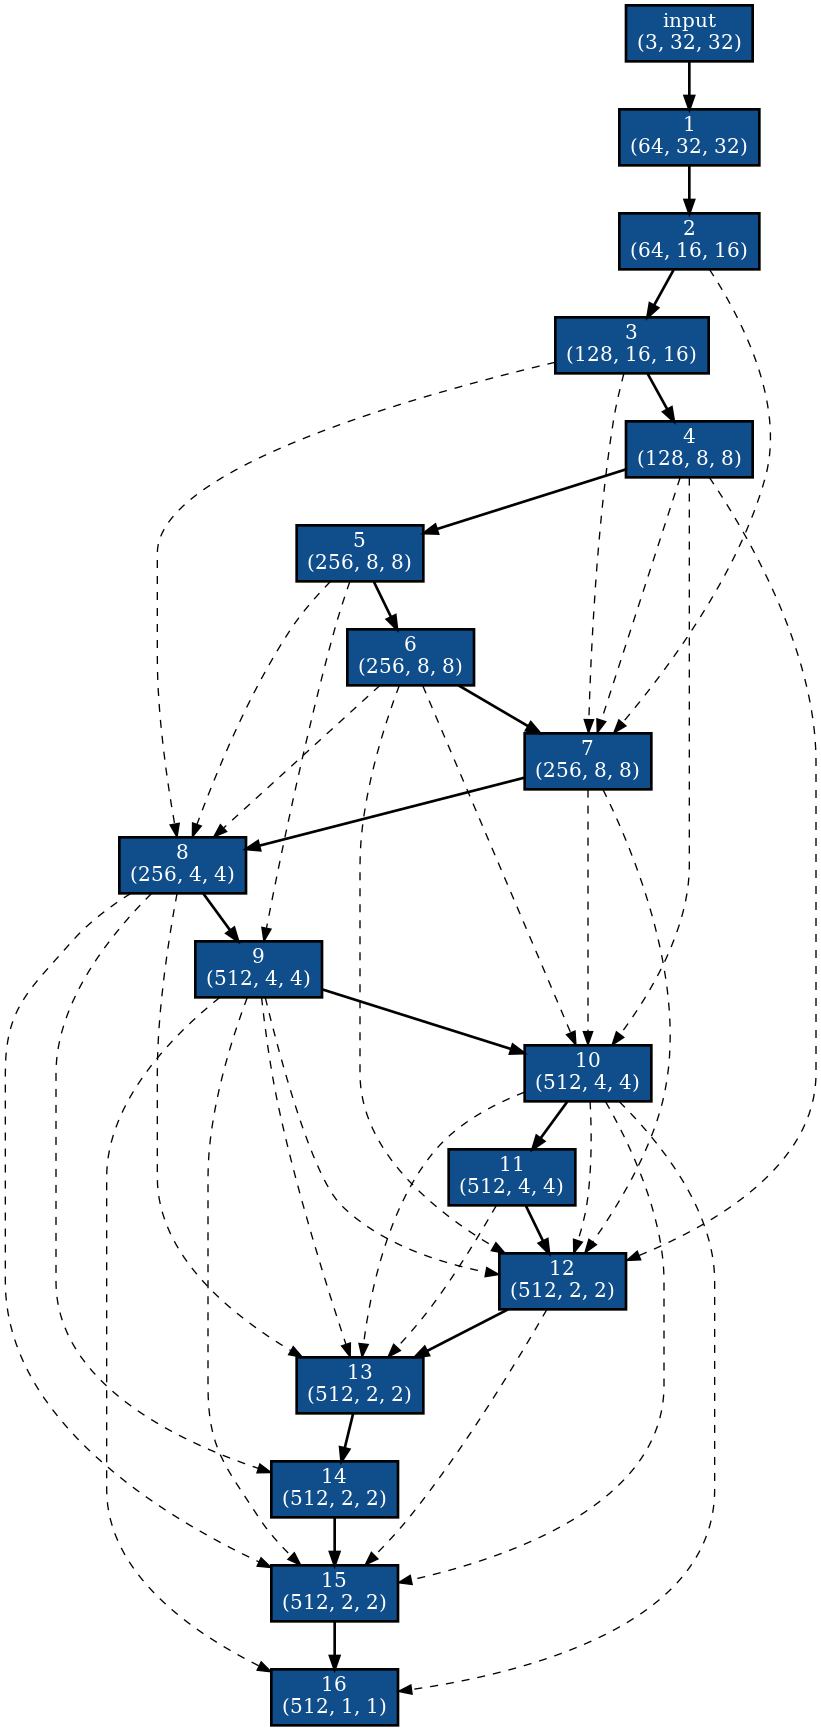
\includegraphics[clip,scale=0.19]{./fig/04.exp/normal_last.png}\\
    DARTS + TDGA ($\bm{\alpha}$)
 	\end{center}
 \end{minipage}
 \begin{minipage}{0.49\hsize}
 	\begin{center}
    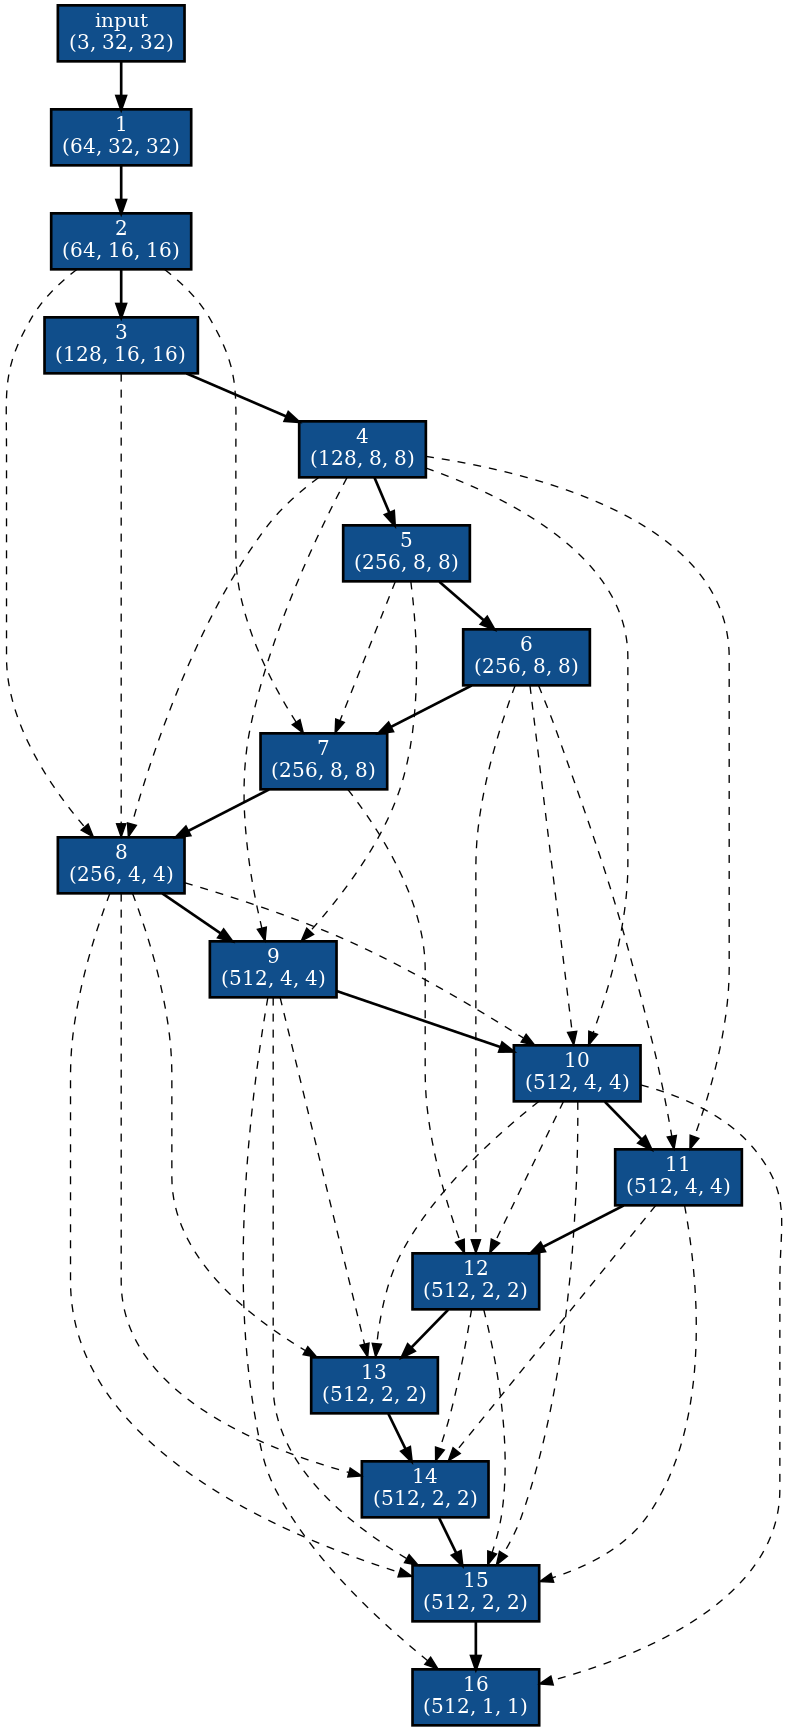
\includegraphics[clip,scale=0.19]{./fig/04.exp/noevo_last.png}\\
    DARTS + TDGA
 	\end{center}
 \end{minipage}
 \caption{実験 2 : 手法のアーキテクチャ 2 / 2}
 \label{fig:exp2/archi2}
\end{figure}

% \begin{figure}[t]
%   \begin{tabular}{cc}
%     \begin{minipage}[t]{0.5\hsize}
%     	\begin{center}
%         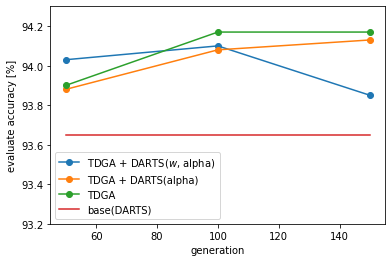
\includegraphics[clip, width=70mm]{./fig/04.exp/eval.png}\\
%         eval
%       \end{center}
%     \end{minipage}
%     \begin{minipage}[t]{0.5\hsize}
%     	\begin{center}
%         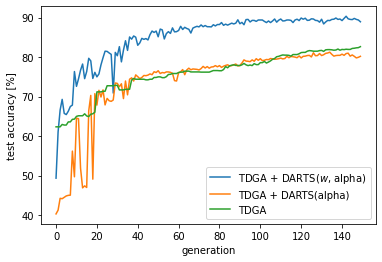
\includegraphics[clip, width=70mm]{./fig/04.exp/acc.png}\\
%         accuracy
%       \end{center}
%     \end{minipage}
%     \\
%     \begin{minipage}[c]{0.5\hsize}
%     	\begin{center}
%         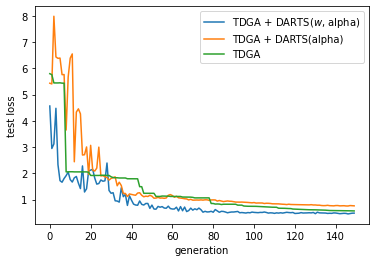
\includegraphics[clip, width=70mm]{./fig/04.exp/loss.png}\\
%         loss
%       \end{center}
%     \end{minipage}
%     \begin{minipage}[c]{0.5\hsize}
%     	\begin{center}
%         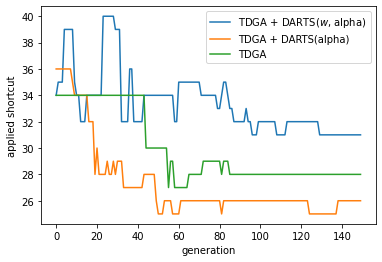
\includegraphics[clip, width=70mm]{./fig/04.exp/edge.png}\\
%         edge
%       \end{center}
%     \end{minipage}
%   \end{tabular}
%   \caption{実験2 : result}
%   \label{fig:exp2_graph}
% \end{figure}
